\documentclass[conference]{IEEEtran}
\IEEEoverridecommandlockouts
% The preceding line is only needed to identify funding in the first footnote. If that is unneeded, please comment it out.
\usepackage{cite}
\usepackage{amsmath,amssymb,amsfonts}
\usepackage{algorithmic}
\usepackage{graphicx}
\usepackage{textcomp}
\usepackage{xcolor}
\def\BibTeX{{\rm B\kern-.05em{\sc i\kern-.025em b}\kern-.08em
    T\kern-.1667em\lower.7ex\hbox{E}\kern-.125emX}}
\begin{document}

\title{A Platform for Searching Texts for Desired Expressions in a User-Editable Pattern Matching Environment for Language Learning\\
%{\footnotesize \textsuperscript{*}Note: Sub-titles are not captured in Xplore and
%should not be used}
%\thanks{Identify applicable funding agency here. If none, delete this.}
}

\author{\IEEEauthorblockN{1\textsuperscript{st} Given Name Surname}
\IEEEauthorblockA{\textit{dept. name of organization (of Aff.)} \\
\textit{name of organization (of Aff.)}\\
City, Country \\
email address}
\and
\IEEEauthorblockN{2\textsuperscript{nd} Given Name Surname}
\IEEEauthorblockA{\textit{dept. name of organization (of Aff.)} \\
\textit{name of organization (of Aff.)}\\
City, Country \\
email address}
}

\maketitle

\begin{abstract}
In this paper we propose a platform of pattern matching system that can extract required phrases or sentences in texts.
Finding certain expressions in texts are often needed in language learning, e.g, examples of case markers
between a predicate and an argument, or possible nouns in subject of a verb in a certain meaning. In previous studies,
several types of systems, containing concordancers, are proposed. However, it is not easy to apply combined
patterns because the pattern mathing templates are previously fixed.
% flexibilityが必要 背景としては task specific な systemで作られているので 英語検索に特化はしてると
% 小論文での表現でみんなが同じようにどう使っているかといった表現の分析に利用するのは容易ではない
% その一番の原因は flexibility 
Thus, we propose a flexible phrase searching system in which users can create search patterns
by combining blocks of basic search templates. % 拡張性がある blockで 提案する
%長すぎる時はここを消す
One of the characteristics the proposed system is that user can also specify where to be highligted
in texts with the blocks.
To realize the function of combining patterns by users, the proposed system employs
Prolog as the base of the data structure. The platform of the searching system is implemented
on an Web server with JavaScript-based interface and database system. 
% ブロックにいろいろ設定することで,ユーザは組み合わせてさらに使うことができる
%To realize the pattern matching of predicate-argument structure, 
%the system emplopys several NLP tools.
In the performance test, we shows that the proposed system can deal with relatively large sclale texts
(10,000 sentences), and also demonstrate the combined patterns can be applied to the texts.
In this paper we discuss the system architecture and the extendability of the pattern matching. 
\end{abstract}

\begin{IEEEkeywords}
  pattern matching, concordancer, browser-based pattern matcher, Prolog
\end{IEEEkeywords}

\section{Introduction}
Extraction of some phrases and expressions in texts is considered essential function in langugage education.
For example, case markers located between a predicate and an object in Japanese language are various
rules and alternations\footnote{The verbs {\it morau} (get) and {\it eru} (obtain) are almost the same meaning
but {\it morau} has alternation between the case markers {\it ni/kara} as {\it kare ni/kara morau}
((I) get (it) from him.), and 
{\it eru} can only takes {\it kara} in this meaning as {\it kare kara/*ni eru}.},
% 彼 から もらう,彼に もらう but, 彼から 得る 彼に 得る.
% もらう,得るの質問 native https://ja.hinative.com/questions/17482159
then language learners need to search for examples of predicate-argument
examples in Japanese texts. 
%also, search for similar phrases in student essays. this is eample for use in education. 
As a tool for searching texts, various kinds of concordancer are proposed, however, 
most concordancers have the liminations in the use of their functionality.
For example, Sketch Engine\footnote{https://www.sketchengine.eu/}, one of the famous concordancers,
proposes Corpus Query Language (CQL)\footnote{https://www.sketchengine.eu/documentation/corpus-querying/}
that has rich templates of pattern maching for words and characters, however, 
most of the templates are mainly effective for English and the templates are realized 
at the level of regular expressions. Thus, users are unable to employ patterns at the level of Context
Free Grammar (CFG) which incorporates dependency parsing or predicate-argument relations.
%predicate object relations with variations of case markers, On the other hand,
From the viewpoint of Natural Language Processing (NLP) research,
dependency parsers (KNP, CaboCha, GiNZA) have already been developed and are available, but it is not easy to
build a pattern matching system with NLP tools from scratch. 

Thus, we propose an environment that users can combine patterns
searching for phrases or expressions in texts without programming.
The system allows users to combine the basic search templates
connected with Prolog predicates that have all of the information
about dependency, POS, and lemmas of sentences analyzed by NLP tools. 
The combination of search templates are consistently composed and the
combined search pattern works to find the intended phrases in texts thanks to
the the Prolog inference engine. 
The system has a browser-based interface based on Blockly\footnote{https://developers.google.com/blockly?hl=ja}
that allows users to combine patterns in a visual environment. 

The contributions of this study are as below:
1) we propose a new type pattern matching system providing the environment in which users can
combine patterns, 
2) Prolog-based search templates allow users flexibility of pattern combinations, and 
3) browser-based system that can be suitable for non-programmers.
In this paper we focus on Japanse pattern matching system because 
most of the concordancers are build for English, and the target of the system is
not only for language learners but also for analysing texts to check the studetnt essays. 

In the performance test, we shows that the proposed system can deal with relatively large sclale texts
(10,000 sentences), and also demonstrate the combined patterns can be applied to the texts.
In this paper we discuss the system architecture and the extendability of the pattern matching. 

\section{Related Studies}

% sketch engine
One of the famous concordancers sketch Engine.
it can seaerch inflections it works effectvenly on English grammars  words, poses can be searched
regular expression grammsars. For English. Japease, word base and keyword list and morphmeme.
Sketch Englihs is tagged corpus and tag and surface are extarctd.

% NPCMJ tregex 
For Japese text search, for language learner, tregex based searching interface in NPCMJ.
they construct Japaennse parsed texts and provide the searchin for syntactical informations
based on annotated tags. They are CFG level concordancer, however, the tools are available only for NPCMJ
text corpus, and it cannot be applied to plan texts.

% text mining
Not for education, but extraction tools in NLP, 
not for language learner, but Chaki is for corpus annotation tool

The is the part of programming, then user is requited to programming skill to use this.


\section{Platfrom of Pattern Matching System}

\subsection{Total View of the Proposed System}
user editable pattern with visual handling, Construction of pattern is not easy, the
user shoud apply the assumed patterns, see the results and then tune up the patterns.
Thus, editing space and results should be exist.

Patterns are combinations, conbining by basic blocks and extract every where matched.
\subsection{Prolog-Based Data Structure in Backend}

\subsection{Example of Patterns}

\section{Performance Tests}

\section{Discussions and Conclusions}


%\section*{Acknowledgments}
%This work was partially supported by JSPS KAKENHI Grant Number 22K00530.


%\begin{table}[htbp]
%\caption{Table Type Styles}
%\begin{center}
%\begin{tabular}{|c|c|c|c|}
%\end{tabular}
%\label{tab1}
%\end{center}
%\end{table}

%\begin{figure}[htbp]
%\centerline{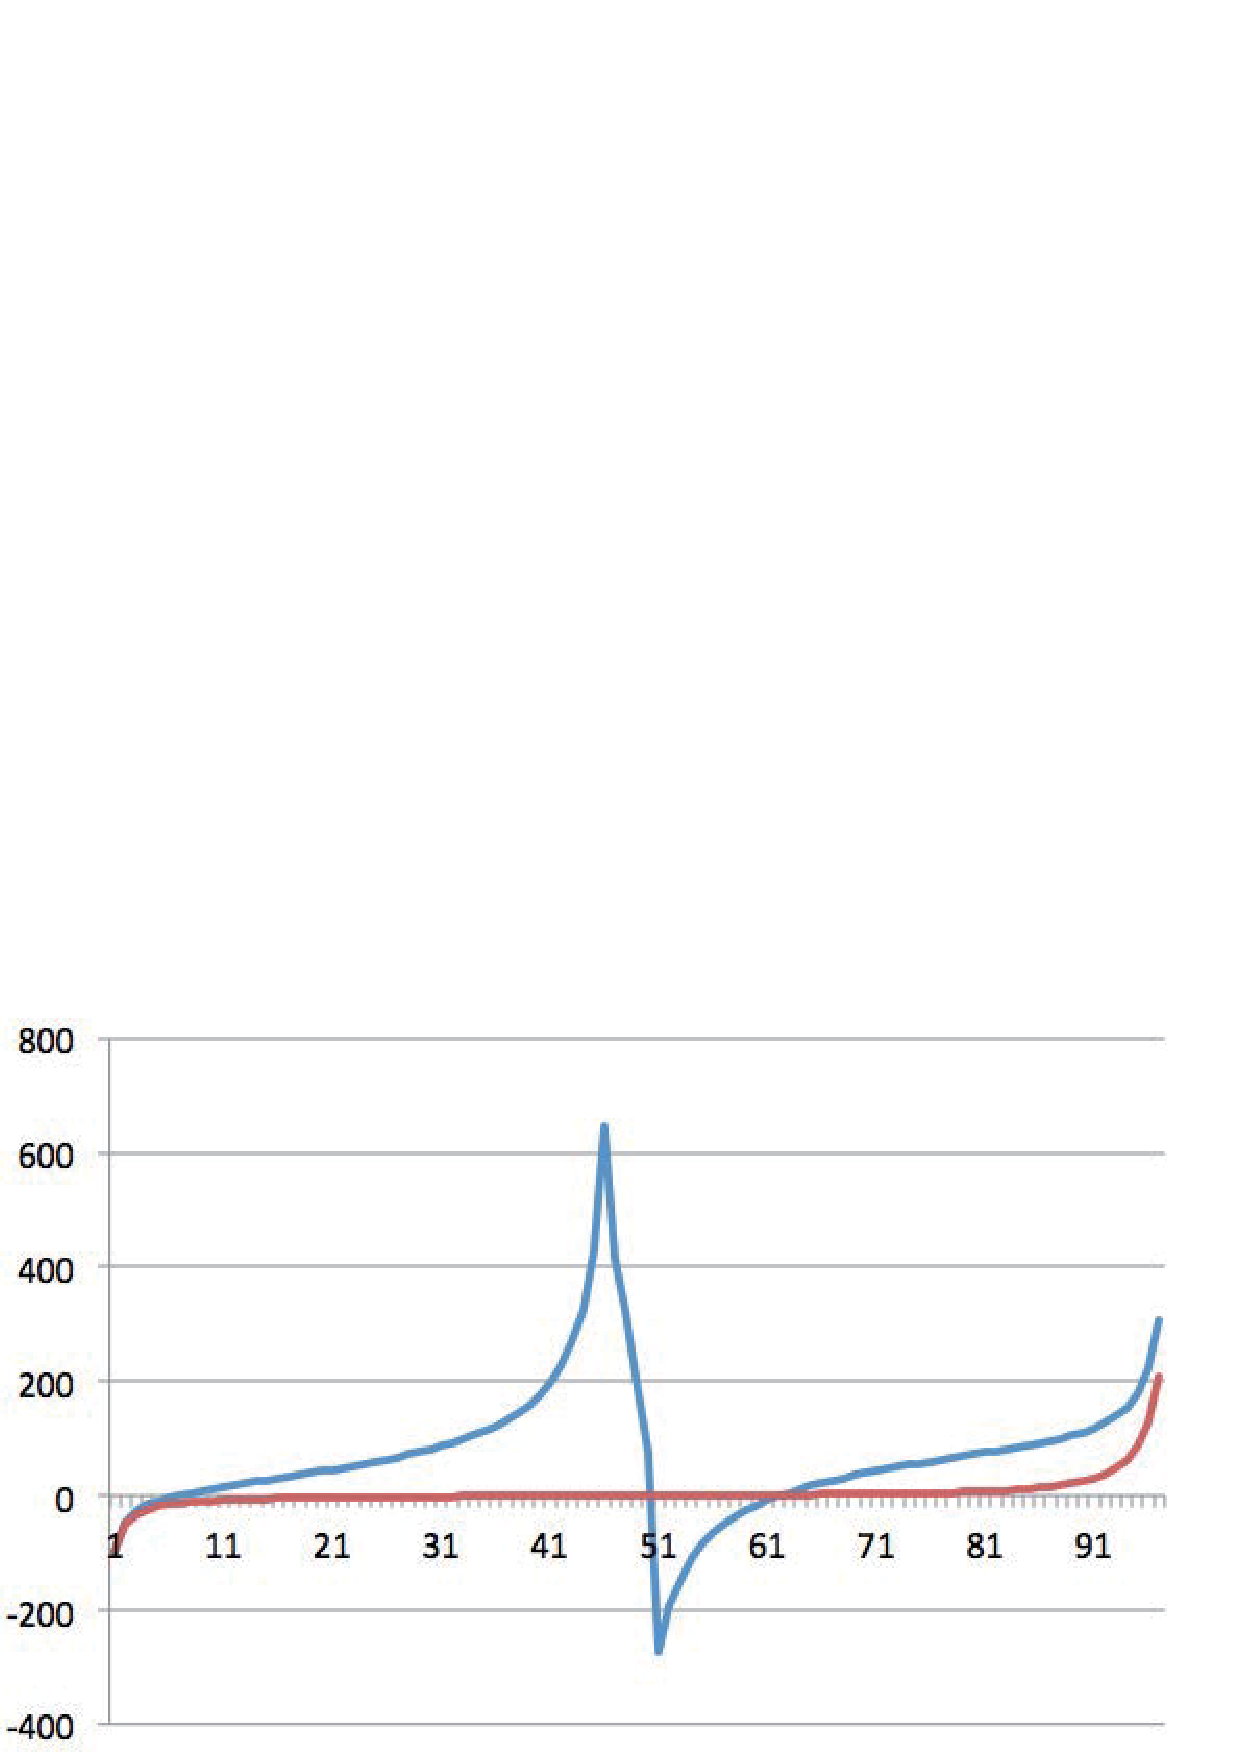
\includegraphics{fig1.png}}
%\caption{Example of a figure caption.}
%\label{fig}
%\end{figure}

\section*{References}


\bibliographystyle{unsrt_abbrv}
\bibliography{all,my-results}

%\begin{thebibliography}{00}
%\end{thebibliography}

\end{document}